\section[Aplicación]{Aplicación web}


Como se estableció en el objetivo de este trabajo, se ha creado una aplicación para recolectar y clasificar noticias, las cuales son mostrados en un entorno web. En esta sección se explica el proceso de funcionamiento de la aplicación web.\\

Para el desarrollo de esta  herramienta se ha utilizado \textbf{Java} para el procesamiento de los datos y para diseñar la vista se ha utilizado: \textbf{HTML}, \textbf{CSS} y \textbf{Java server faces}, ademas para conectar el proceso de recolección y clasificación (escritos en \textbf{Python 3}) se hecho uso de \textbf{subprocesos}, los cuales son procesos que corren en segundo plano.\\

La aplicación esta diseñada en 4 etapas, las cuales son mostradas en la Figura \ref{fig:procesoAppWeb}, donde la etapa \textbf{Selección} describe las secciones disponibles para obtener noticias; la etapa \textbf{Recolectar} muestra la integración de los \textit{crawlers} en la herramienta; la etapa \textbf{Clasificar} hace uso del modelo clasificador desarrollado en la sección anterior y para concluir, la etapa \textbf{Mostrar resultados} describe la forma en que los datos son presentados al usuario. Es importante mencionar que las etapas en color azul cielo siempre son ejecutadas, sin embargo las de color gris no siempre son llevadas acabo. A continuación se explica a detalla cada una las tareas.


\begin{figure}[H]
	\centering
	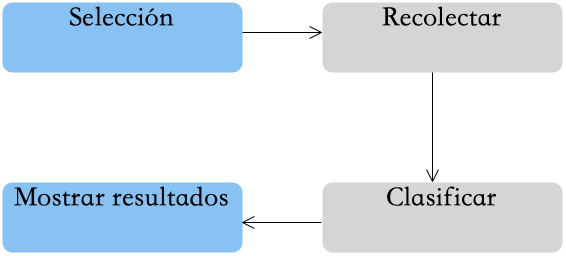
\includegraphics[scale=0.6]{imagenes/Capitulo5/AplicacionWeb/ProcesoAplicacionWeb.png}
	\caption{Etapas de la aplicación web}
	\label{fig:procesoAppWeb}
\end{figure}

%
% este proceso se llevará a cabo la primera vez que se seleccione una sección o en el caso de que %hayan transucurrido 4 horas de la última vez que se utilizó el sistema.%
%\\%
%
%\begin{figure}[H]
%	\centering
%	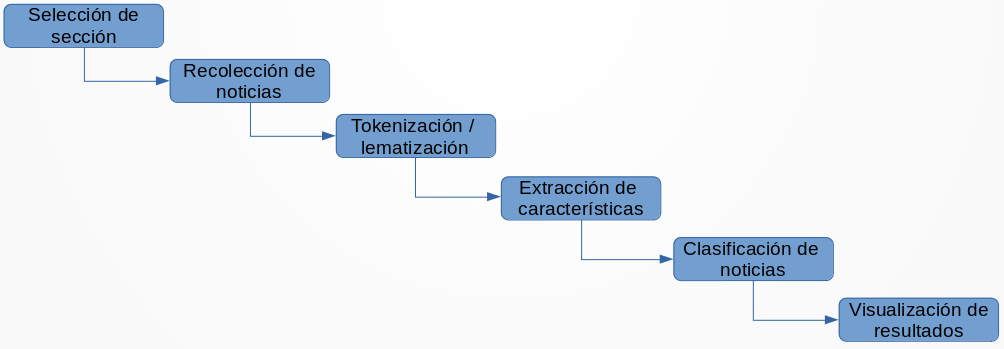
\includegraphics[scale=0.3]{imagenes/Capitulo5/procesoRecoleccionClasificacion.png}
%	\caption{Etapas de la aplicación web}
%	\label{fig:procesoAppWeb}
%\end{figure}
%

\subsection{Selección}


Esta etapa permite elegir al usuario la sección de noticias a buscar. La aplicación comienza en una pantalla inicial, donde se muestra un menú con las opciones \textbf{Inicio}, \textbf{Cultura}, \textbf{Deportes}, \textbf{Economía}, \textbf{Política}, \textbf{Ciencia y Tecnología}, estas categorías (excluyendo \textbf{Inicio}) son las secciones permitidas para recolectar noticias, como se muestra la el Figura \ref{fig:PantallaInicio}. Cabe mencionar que la opción \textbf{Inicio}, permite regresar a la pantalla principal.\\


\begin{figure}[H]
\centering

\includegraphics[scale=0.35]{imagenes/Capitulo5/pantallaPrincipal.png}
\caption{Pantalla de Inicio}
\label{fig:PantallaInicio}
\end{figure}

Después de elegir una sección, se muestra el mensaje \textbf{En proceso de recolección y clasificación}, como se visualiza en la Figura \ref{fig:loading}, el cual informa que las etapas \textbf{Recolectar} y \textbf{Clasificar} están en proceso, además cuando se muestra este mensaje no se puede seleccionar otra secciones hasta que el proceso concluya. Cabe destacar que el proceso continua de forma normal si se cumplen las siguientes condiciones:

\begin{enumerate}
	\item \textbf{Primera vez}: Esta condición hace referencia a la etapa \textbf{selección}, es decir cuando es la primera vez que se ha selecciona una sección, se debe proceder con las siguientes etapas

	\item \textbf{Límite de periodo}: Esta condición define 4 horas como el periodo de recolección, es decir cuando se ha solicitado mostrar las noticias de una sección y ha transcurrido 4 horas desde la última petición (Ver regla de negocio \RNref{RN8}{Periodo de actualización}), se debe proceder con las siguientes etapas
\end{enumerate}	

Como consecuencia de no cumplirse estas condiciones, las etapas \textbf{Recolectar y Clasificar} no son iniciadas, debido a que los artículos con su clasificación correspondiente se encuentran almacenados en el sistema, por esta razón se procede directamente con la etapa \textbf{Mostrar resultado}.

\begin{figure}[H]
\centering
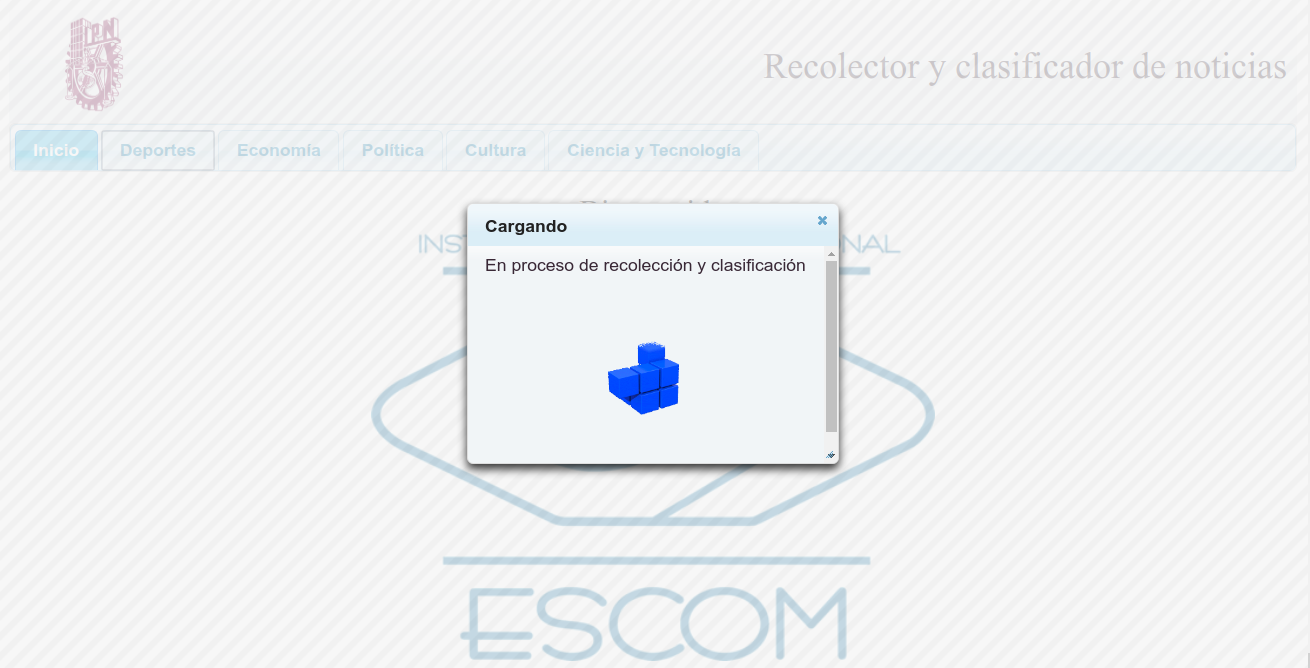
\includegraphics[scale=0.35]{imagenes/Capitulo5/mensajeEspera.png}
\caption{Mensaje de espera}
\label{fig:loading}
\end{figure}


\subsection{Recolectar}


Esta etapa genera un subproceso el cual activa un script (desarrollado en \textbf{Python 3}) el cual inicia la recolección de noticias en los sitio web definidos previamente (ver \Tref{cp5:sitiosWeb}{Sitios web}), la información que se obtiene de cada artículo es la siguiente:

\begin{itemize}
	\item \textbf{URL de la noticia}
	\item \textbf{Título}
	\item \textbf{Fecha}
	\item \textbf{Autor}
	\item \textbf{Descripción} (Existen sitios web, donde las noticias no cuentan con una descripción)
	\item \textbf{Noticia}
\end{itemize}

La extracción de las noticias se hace en la página principal de los sitios web. Cabe destacar que en el proceso de recolección se valida que las noticias contengan al menos 180 palabras (en la redacción de \textbf{Noticia}), de lo contrario no se extrae. Ademas se ha definido un tiempo máximo de espera en esta etapa, el cual es de 30 segundos, después de concluir el periodo y haber recolectado la información, se procede con la etapa de \textbf{Clasificación}, de lo contrario si no se recolecto ninguna noticia se muestra el mensaje \textbf{Se ha agotado el tiempo de espera, no se han encontrado noticias, intentar mas tarde} (como se visualiza en la Figura \ref{fig:notNoRec}) y se detiene el proceso.

\begin{figure}[H]
\centering
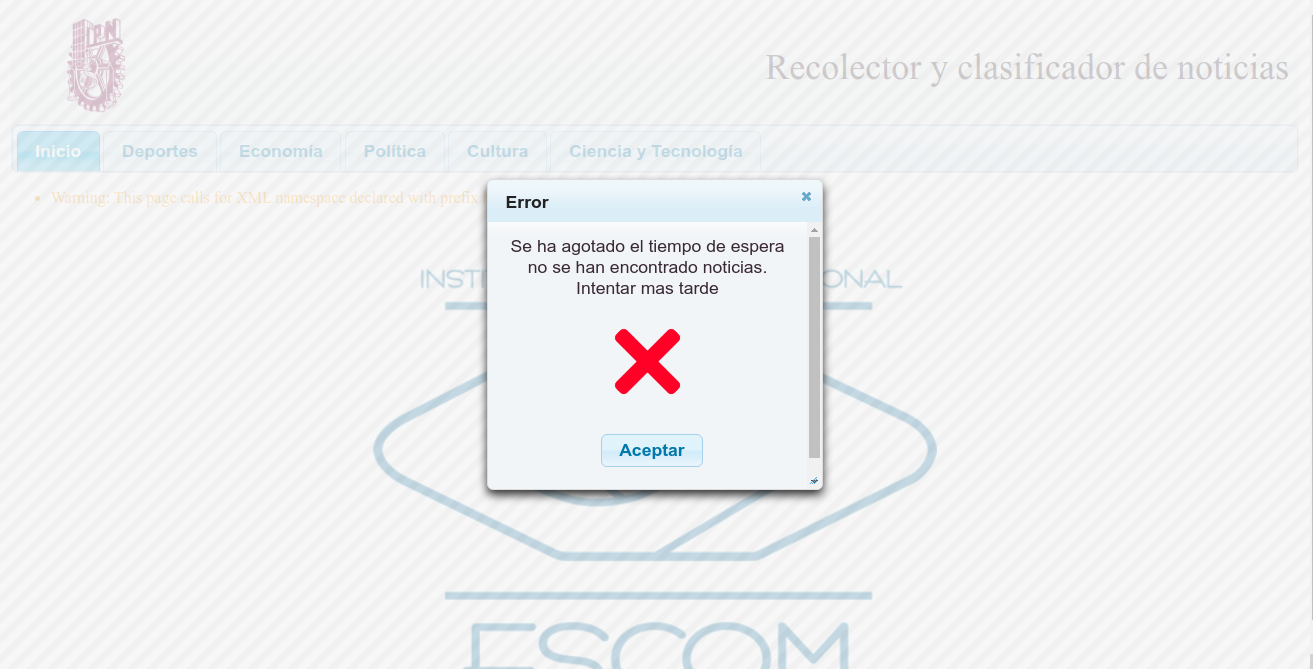
\includegraphics[scale=0.3]{imagenes/Capitulo5/errorConectividad.png}
\caption{Mensaje de error en la recolección}
\label{fig:notNoRec}
\end{figure}

\subsection{Clasificar}

Después de recolectar las noticias se inicia la etapa de clasificación, el cual esta conformado por 5 tareas (como se muestra en la Figura \ref{fig:cp5:clasificacion}). Esta etapa genera un subproceso para ejecutar un script desarrollado en \textbf{Python 3}, el cual está encargado de llevar acabo cada tarea de esta sección. Cabe destacar que el proceso de clasificación solo utiliza el contenido de la noticia, los demás datos no son necesarios en esta etapa. A continuación se explica cada subtarea.

\begin{figure}[H]
\centering
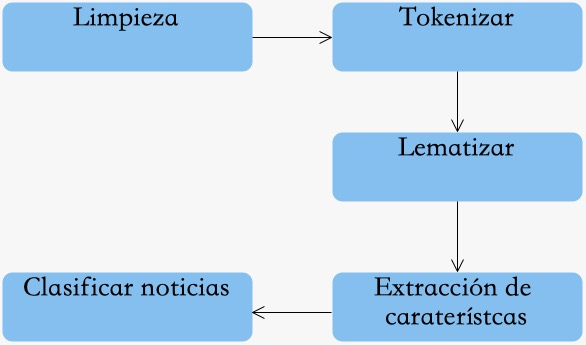
\includegraphics[scale=0.5]{imagenes/Capitulo5/AplicacionWeb/PreprocesamientoWeb.png}
\caption{Proceso de clasificación}
\label{fig:cp5:clasificacion}
\end{figure}

\begin{enumerate}

	\item \textbf{Limpieza}: En la sección de \textbf{Entrenamiento} el proceso de limpieza (ver \Tref{cp5:limpieza}{Limpieza}) consiste en eliminar texto que no brinda información útil como, hipertexto (ver \Tref{cp3:html}{HTML}), símbolos especiales (como \# $\dagger$ $\sqrt{ }$), \textit{emojis} (como \dSmiley \dCooley \dNinja), sin embargo en esta etapa no es necesario hacer esta limpieza, debido a que el vocabulario definido no contiene estos datos, por esta razón estos símbolos son ignorados en la extracción de características. Cabe señalar que lo único que es eliminado son los saltos de línea

	\item \textbf{Tokenizar}: Consiste en separar el texto en sus elementos mínimos por un espacio (ver \Tref{cp5:tokenizacion}{Tokenizar})

	\item \textbf{Lematizar}: Proceso que reduce cada una de las palabras tokenizadas en lemas(ver \Tref{cp5:lematizacion}{Lematizar})

	\item \textbf{Extracción de características}: Se extrae palabras (características) con base al vocabulario definido al final de la etapa de entrenamiento (ver \Tref{cp5:persistencia}{Persistencia}), para crear un espacio vectorial por cada noticia (esta es la representación que el algoritmo entiende). Cabe destacar que las características son extraídas de forma binaria (ver \Tref{cp5:extraccion}{Extracción de características})

	\item \textbf{Clasificar}: Al final de la sección \textbf{Entrenamiento} se almacenó el modelo clasificador (ver \Tref{cp5:persistencia}{Persistencia}) el cual esta basado en el algoritmo \textbf{Maquinas de soporte vectorial} (ver \Tref{cp3:msv}{MSV}). Esta tarea utiliza el clasificador el cual recibe como entrada los vectores de características(los cuales representan el contenido de cada artículo) y como salida brinda la clasificación del conjunto de noticias, y son almacenadas por sección en un archivo \textbf{CSV}

\end{enumerate}


\subsection{Mostrar resultados}

Esta etapa consiste en presentar el resultado del proceso de clasificación en la herramienta. Cuando este proceso ha concluido se muestra el mensaje \textbf{Noticias listas para ser mostradas}, donde el usuario tiene la opción de elegir visualizar las noticias o cancelar el flujo del sistema, como se muestra en la Figura \ref{fig:notClass}.

\begin{figure}[H]
\centering
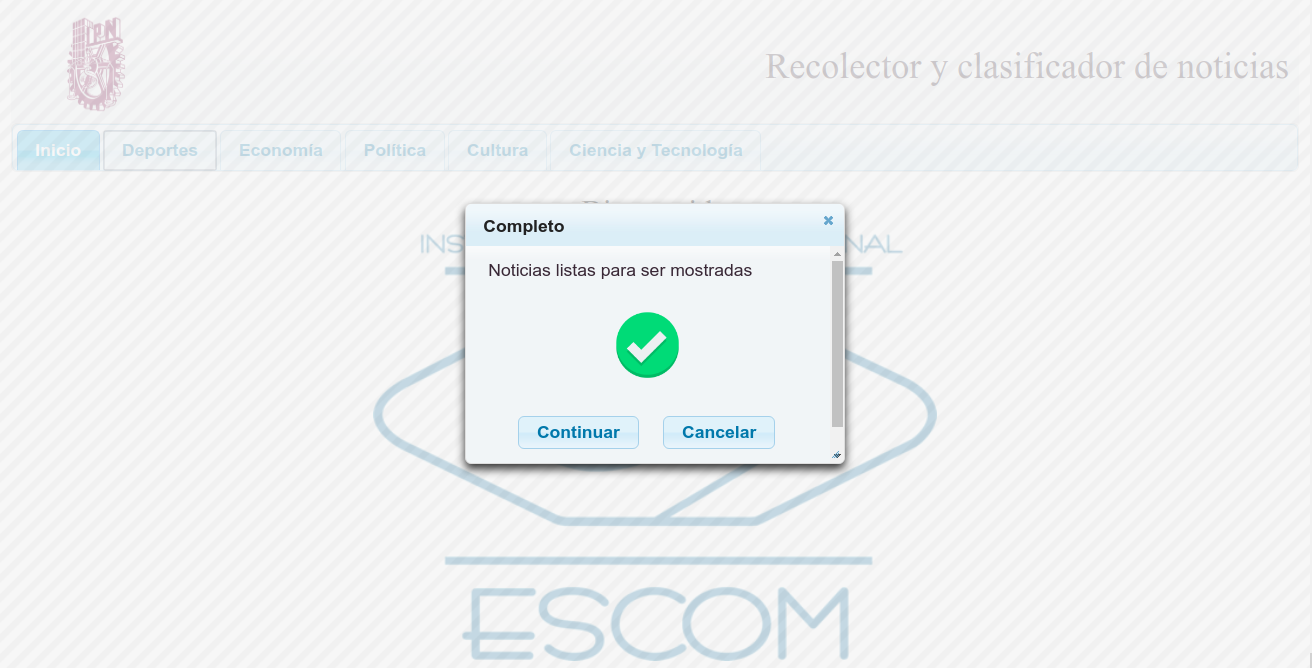
\includegraphics[scale=0.35]{imagenes/Capitulo5/noticiasListasParaSerMostradas.png}
\caption{Mensaje que se muestra una vez clasificadas las noticias}
\label{fig:notClass}
\end{figure}

Si el usuario ha presionado la opción \textbf{Cancelar}, el proceso concluye y la herramienta muestra la Pantalla de Inicio (ver \ref{fig:PantallaInicio}), de lo contrario si se ha dado clic en \textbf{continuar}, se lleva acabo el proceso mostrado en la Figura \ref{fig:cp5:mostrar}, las tareas en color azul cielo siempre son llevadas acabo y las de color gris son opcionales. A continuación estas etapas son descritas.

\begin{figure}[H]
\centering
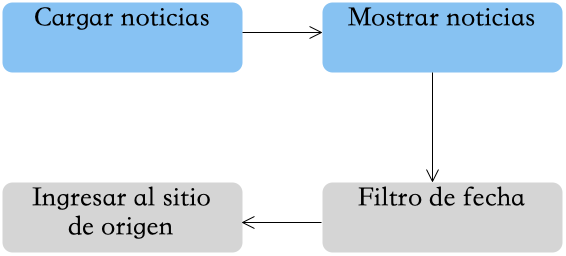
\includegraphics[scale=0.55]{imagenes/Capitulo5/AplicacionWeb/MostrarDatosApp.png}
\caption{Funcionalidad de la aplicación}
\label{fig:cp5:mostrar}
\end{figure}


\begin{enumerate}

	\item \textbf{Cargar noticias}: En el proceso de clasificación se crea un archivo \textbf{CSV} por cada sección con las noticias correspondientes, en esta etapa se obtiene los artículos de la sección elegida por el usuario

	\item \textbf{Mostrar noticias}: En la pantalla principal, las noticias se muestran por fecha de publicación, los datos mostrados por cada noticia son: \textbf{título de la noticia}, \textbf{resumen de la noticia}(de contar con ello), \textbf{autor} y finalmente la \textbf{fecha de publicación}. Como se muestra en la Figura \ref{fig:vistaNoticias}


	\item \textbf{Filtro fecha}: En la sección de las noticias, se muestra un menú con las opciones: \textbf{Hoy}, \textbf{Ayer}, \textbf{Dos días} y \textbf{Tres días o mas}. Este es una herramienta que permite filtrar los artículos por fecha de publicación. Por ejemplo, si el usuario desea visualizar noticias de un día anterior a la registrada por el sistema, se debe seleccionar la opción \textbf{Ayer}, en seguida la información de este periodo se muestra, como en la Figura \ref{fig:vistaNoticiasAyer}. Es importante mencionar que las noticias mostradas por defecto son las del día de consulta (\textbf{Hoy})

	\item \textbf{Ingresar al sitio de origen}: Cada noticia mostrada contiene la \textbf{URL} al sitio de origen de la noticia, si el usuario desea leer el artículo completo se debe dar clic en la noticia y la aplicación redirige el buscador a la pagina fuente

\end{enumerate}


\begin{figure}[H]
\centering
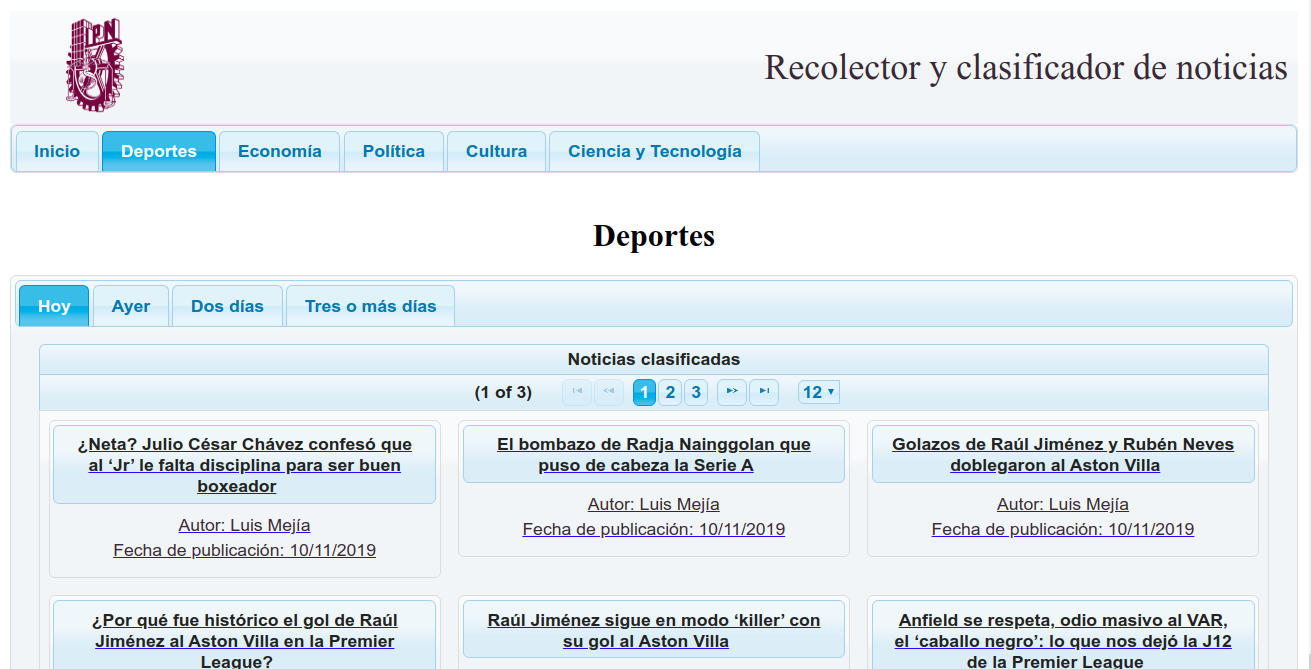
\includegraphics[scale=0.45]{imagenes/Capitulo5/noticiasDeHoy.png}
\caption{Vista de las noticias recolectadas}
\label{fig:vistaNoticias}
\end{figure}




\begin{figure}[H]
\centering
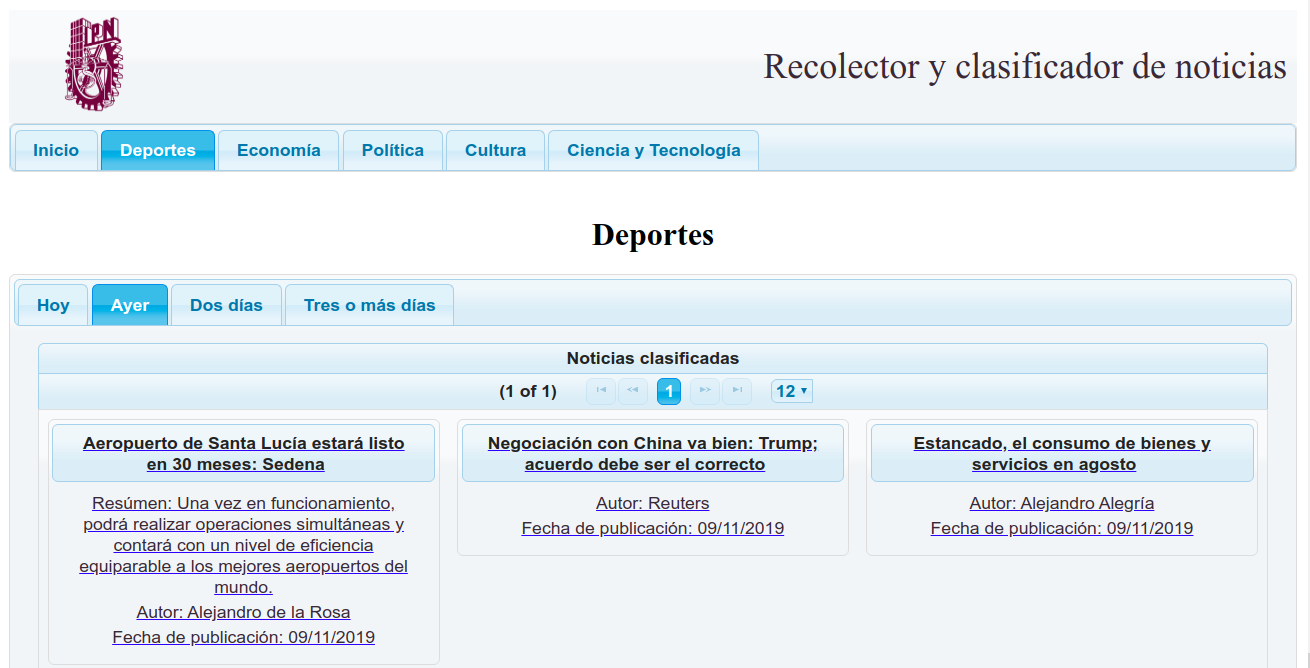
\includegraphics[scale=0.45]{imagenes/Capitulo5/noticiasDeAyer.png}
\caption{Vista de las noticias recolectadas del día de ayer}
\label{fig:vistaNoticiasAyer}
\end{figure}

